% Dossier des interfaces de communication
% Version 1.0

% Historique des versions
% 01/02/08 0.1 Document LaTex et premier jet du plan
% 01/02/08 0.2 Intro et rappel de l'architecture globale
% 05/02/08 1.0 Version relue et validée

\documentclass[a4paper, 11pt, final]{article}

\usepackage[utf8]{inputenc} % Texte en utf-8
\usepackage[cyr]{aeguill} % Coupure des mots accentués
\usepackage[francais]{babel} % Typographie française
\usepackage[pdftex, hypertexnames=false, colorlinks=true, final]{hyperref}
\usepackage[final]{graphicx}
\usepackage{url} % Gestion des URLs
\usepackage{geometry}
\usepackage{fancyhdr}
\usepackage[Lenny]{fncychap}

% Marges à gauche et à droite de 3cm
\geometry{margin=3cm}

% Utilisation des headers et footers personnalisés de fancyhdr
\pagestyle{fancy}

% Images dans le dossier ./images/
\graphicspath{{./images/}}

% Gestion des métadonnées étranges à rendre visibles au rendu
\newcommand\docname{DICv1.0}
\newcommand\docauthor{Nicolas Kandel -- Rémi Thévenoux}
\newcommand\docstatus{LIVRABLE} % EN COURS, ATTENTE, VALIDE ou LIVRABLE

% Numérotation mieux
%\renewcommand\thechapter{\Alph{chapter}}
%\renewcommand\thesection{\Roman{section}}
%\renewcommand\thesubsection{\arabic{subsection}}
%\renewcommand\thesubsubsection{\alph{subsubsection}}

% Format de citation de références standard, marche avec quasiment tout
\newcommand\fullref[1]{\ref{#1}, page \pageref{#1}}

% En-têtes et pieds de page
\lhead{\docname}
\lfoot{Auteur : H4213}
\cfoot{}
\rfoot{\thepage}

% Titre du document maître
\title{\textbf{COPEVUE}\\
\rule{\textwidth}{1pt}{}\\
\Huge{\textsc{Dossier des interfaces de communication}}}
\author{\docauthor{} (H4213)}
\date{\docname{} --- \today{} (\docstatus{})}

\begin{document}

\maketitle

\tableofcontents

\pagebreak

\section{Introduction}

\subsection{Rappel du contexte}
Il existe aujourd'hui de nombreux sites isolés et/ou difficiles d'accès
qui nécessitent une surveillance et parfois des actions à distance.
Ces sites se situent dans des espaces très différents tels que les
citernes placées dans les forêts escarpées du pourtour méditerranéen,
les réservoirs utilisés pour l'autonomie des chantiers dans le grand
Nord mais aussi les personnes âgées qui se retrouvent souvent isolées.

Actuellement tous les contrôles et actions sont réalisés par un opérateur
qui doit se déplacer sur le site.
Il n'y a donc que très peu de réactivité, on ne peut pas avoir un suivi
fin des évolutions et des problèmes graves~--par exemple la fuite d'un
réservoir~-- ne peuvent pas être traités rapidement.

\paragraph{Étude COPEVUE}
L'objet de l'étude est la mise en place d'un système générique de
surveillance et d'action à distance sur des sites isolés.
Le système devra être évolutif, autonome et fiable.

\subsection{Présentation du document}
Ce document ~-- Dossier des interfaces de communication~-- définit de
façon exhaustive l'ensemble des communications établissables entre les
différents acteurs du système ainsi que les interfaces mises en jeu.

\subsection{Documents applicables et de référence}
\paragraph{Documents applicables}
\begin{itemize}
\item Dossier de gestion de la documentation
\item Dossier de spécification technique des besoins
\item Dossier de faisabilité
\end{itemize}

\paragraph{Documents de référence}
\begin{itemize}
\item Plan de référence d'un dossier d'interfaces de communication
\end{itemize}


\section{Rappel de l'architecture à déployer}
% On reliste tout ce qui existe pour après dire qui communique avec qui et comment

\subsection{Rappel des différents acteurs}
% Acteurs
    Afin de cibler parfaitement les différentes interfaces de communication que
nous allons présenter, voici un un rappel des différents acteurs qui rentrent en
compte dans notre système. Ceux-ci sont découpés en six sous-systèmes distincts
et relativement indépendants :

\begin{description}
    \item[Le site isolé] correspond à l'ensemble du matériel et de
    l'applicatif des sites isolés en dehors de l'alimentation énergétique.
    \item[L'alimentation énergétique] est le système permettant de fournir
    l'énergie aux sites isolés.
    \item[Le système central] est le système où sont stockées toutes les données
    et où sont effectués les traitements de celles-ci.
    \item[Le poste de gestion] est le poste permettant de configurer le système
    central ainsi que de visualiser des données.
    \item[Le système de l'intervenant] est le système permettant à l'intervenant
    de recevoir et d'envoyer des informations pendant ses interventions.
    \item[Le système de communication] est le système permettant la communication
    entre le système central, les sites isolés et le système de l'intervenant.
\end{description}

\subsection{Rappel de l'architecture globale}
Les différents sous-systèmes~-- aussi appelés acteurs~-- rappelés ci-dessus sont
reliés entre eux selon le schéma global suivant :
% Schéma
\begin{figure}[!h]
\begin{center}
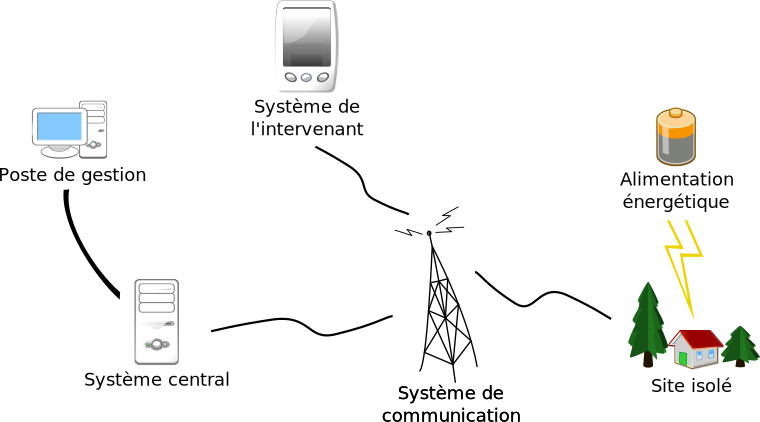
\includegraphics[width=\textwidth]{schema_architecture_generale.png}
\caption{Architecture générale}
\end{center}
\end{figure}

\section{Communications entre sous-systèmes}
% Liste les différentes communication que l'on prévoit entre acteur (exhaustif)
% liste ou tableau ou schéma ?

\subsection{Principe}
Tous les sous-systèmes n'ont pas besoin de communiquer entre eux.
L'\emph{alimentation énergétique} ne communique avec aucun autre acteur,
on considérera la consultation des capteurs à l'initiative du \emph{site
isolé} comme une simple demande de données~-- l'\emph{alimentation énergétique}
faisant partie du \emph{site isolé}, elle en a été dissociée pour des
raisons logistiques.

De plus, le \emph{système de communication} n'est pas un acteur comme
les autres. Son unique but et de relayer les informations et d'assurer
la communication entre sous-systèmes distants.

Les potentielles communications à établir entre sous-systèmes sont prédéfinis.
Par exemple, il n'y a aucun intérêt à permettre au \emph{système de l'intervenant}
de se connecter directement au \emph{poste de gestion}~-- cela serait même une
potentielle faille de sécurité.

\paragraph{}
Voici la liste exhaustive des communications qui sont à prévoir :
\begin{itemize}
\item Système central $\leftrightarrow$ Couche applicative spécifique
\item Poste de gestion $\rightarrow$ Système central
\item Système central $\leftrightarrow$ Site isolé
\item Système de l'intervenant $\rightarrow$ Site isolé
\item Système de l'intervenant $\leftrightarrow$ Système central
\end{itemize}

% Rajouter un schéma tout beau ?
On précise que l'ensemble de ses communications se font de façon asynchrone.


\subsection{Poste de gestion $\rightarrow$ Système central}
Le poste de gestion se connectera au système central grâce au protocole SSH.
Une fois la connexion établie, le poste de gestion pourra alors directement
récupérer les fichier XML où sont stockées les données enregistrées par le
système central. Le poste de gestion pourra aussi accéder et modifier
directement les différents fichiers de configuration, que ce soit les DTD
décrivant les XML, les fichiers de configuration des différentes applications
ou encore le serveur de courriel.

% quid des applications de statistique ?


\subsection{Système central $\leftrightarrow$ Site isolé}
Deux cas se présentent :

\begin{itemize}
\item Le système central désire récupérer des données, utiliser des actionneurs
ou configurer un site isolé. Dans ce cas le système central établit une
connexion via SSH avec le site isolé. Une fois connecté, il
peut alors directement récupérer les données stockées sur le site isolé,
utiliser les différents actionneurs ou encore modifier la configuration
du site isolé.
\item Le site isolé veut envoyer un message au système central. Pour cela
il enverra un courriel au système central, la définition de son contenu
sera liée à l'applicatif présent sur le système central. Dans le cas de la Norvège,
les sites isolés ne pourront envoyer des courrielf que s'ils détectent une anomalie.
Le courriel contiendra le numéro de l'anomalie détectée, l'horaire de détection
ainsi qu'un couple composé du numéro de capteur~-- ou actionneur~-- et de sa valeur.
\end{itemize}


\subsection{Système de l'intervenant $\rightarrow$ Site isolé}
L'intervenant peut se connecter au site isolé à distance ou sur place. À distance il utilisera la connexion GPRS de son \textit{smartphone} pour se connecter en SSH au site en question. Celui-ci dispose d'une paire clef public/privée afin de permettre une authentification RSA. Le principe est le même pour une connexion sur place où l'intervenant utilisera une interface USB et toujuours une authentification RSA.

Toutes les communications entre le système de l'intervenant et les sites isolés se font à sens unique et à l'initiative du système de l'intervenant.


\subsection{Système de l'intervenant $\leftrightarrow$ Système central}
Les communications entre l'intervenant et le système central se font principalement par
échange de courriels et par échange de données sur le modèle client/serveur.

Lorsque le PDA a des requêtes à adresser au serveur~-- demande d'itinéraire~-- il interroge le serveur HTTP du système central avec un URL spécifique. Ces requêtes peuvent nécessiter des informations passées en paramètres par l'émetteur~-- position de l'intervenant, etc. Après traitement de la requête par le système central, le serveur web retourne les informations nécessaires au système initiateur de la requête.

Toutes les autres communications de type notification~-- message, position, etc.~-- se feront par l'envoi de courriels. Du coté du système de l'intervenant, un module de communication s'occupe de la réception et de l'envoi de ces courriels. C'est ce module qui redistribue les messages reçus aux autres modules applicatifs installés sur le \textit{smartphone}, et c'est par lui que passent tout les messages devant être envoyés au système central. Le système central dispose d'un serveur de courriels qui réceptionnera les messages du système de l'intervenant et lui en enverra le cas échéant. Le serveur de courriels se situant sur le système central est dédié exclusivement à cette tâche afin de minimiser le temps de traitement. Ce sont les applications elles-mêmes qui iront chercher les courriels leur étant destinés.

\section{Description des interfaces}

\subsection{Système central $\leftrightarrow$ Couche applicative spécifique}
Le système central est découpé en différentes couches qui seront
développées indépendamment mais communiqueront grâce à une API normalisée.

\paragraph{}
La couche basse fournit les services suivant à l'applicatif spécifique présent sur le système central :
\begin{itemize}
\item \texttt{long lire(siteId leSiteIsole, capteurId leCapteur)}
Service qui permet de lire la valeur d'un capteur situé sur un site isolé.
La valeur du capteur sera transférée sous forme d'un \texttt{long} (8 octets).
\item \texttt{int actionner(siteId leSiteIsole, actionneurId lActionneur, long laConsigne)}
Ce service permet d'utiliser un actionneur, la consigne assignée à l'actionneur
sera codé sur un \texttt{long} (8 octets). Le service retourne un code d'erreur sur un
\texttt{integer} (4 octets).
\item \texttt{int configurer(siteId leSiteIsole, fichier leFichierdeConfig)}
Ce service permet la configuration d'un site isolé. Pour cela il prend en
paramètre un fichier XML de configuration qui décrit l'ensemble des valeurs
et paramètres à configurer sur le site isolé. Le service retourne un code
d'erreur sur un \texttt{integer} (4 octets).
\end{itemize}

\paragraph{}
La deuxième fonction de la couche basse est de récolter automatiquement les données sur les sites isolés. Ces données sont stockées dans des fichiers XML dont la structure est définie par une DTD. Le fichier de DTD à utiliser, la périodicité de relevé des données et toutes les autres informations nécessaires seront définies dans un fichier de configuration en XML. Tous les fichiers de données XML ayant utilisé le même document DTD seront stockés dans le même dossier qui contiendra la DTD en question.

\subsection{Site isolé}
L'interface proposée par les sites isolés est composée des commandes suivantes :
\begin{itemize}
\item \texttt{captor read <id-capteur>}
\item \texttt{captor list}
\item \texttt{captor add <id> <type> <description>}
\item \texttt{captor remove <id>}
\end{itemize}

\paragraph{}
\begin{itemize}
\item \texttt{action do <id> value}
\item \texttt{action list}
\item \texttt{action add <id> <type> <description>}
\item \texttt{action remove <id>}
\end{itemize}

\paragraph{}
\begin{itemize}
\item \texttt{config list}
\item \texttt{config write <variable> <value>}
\item \texttt{config delete <variable>}
\end{itemize}

\end{document}
